Se desarrollan 4 modelos: un modelo ARIMA como base de comparación, un modelo LSTM, un modelo CNN y un híbrido LSTM-CNN.

\section{ARIMA}
Los modelos ARIMA (Autoregressive Integrated Moving Average) son una tipo de modelos estadísticos utilizados históricamente para el análisis y la predicción de series temporales
univariable. 

Utilizamos como base de comparación los resultados de un ARIMA para cada serie temporal: cada variable en cada ubicación y cada fuente de datos.

Para emplear un modelo ARIMA, es necesario ajustar cada uno de sus parámetros, que son:
\begin{itemize}
    \item $p$: el número de términos autorregresivos (AR).
    \item $d$: el número de diferencias necesarias para hacer la serie estacionaria (I).
    \item $q$: el número de términos de media móvil (MA).
\end{itemize}

\subsection{Calibración de términos autorregresivos}
Para determinar el número de términos autorregresivos, se utiliza la función \texttt{plot\_pacf} de la librería \texttt{statsmodels}, 
que permite visualizar la función de autocorrelación parcial (PACF) de la serie temporal. Observamos ejemplos de los resultados en las figuras \ref{arima_pacf_hum}, \ref{arima_pacf_pres}. 

\begin{figure}[H]
    \centering
    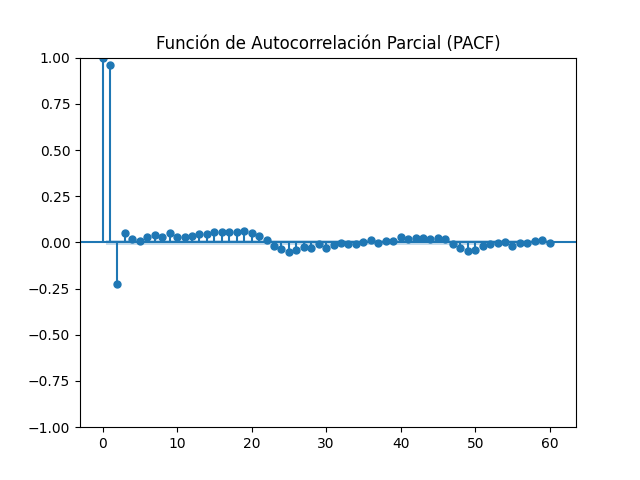
\includegraphics[width=0.5\textwidth]{images/arima_pacf_hum.png}
    \caption{Gráfico de PACF para la serie de humedad relativa en La Laguna de Grafcan}
    \label{arima_pacf_hum}
\end{figure}

\begin{figure}[H]
    \centering
    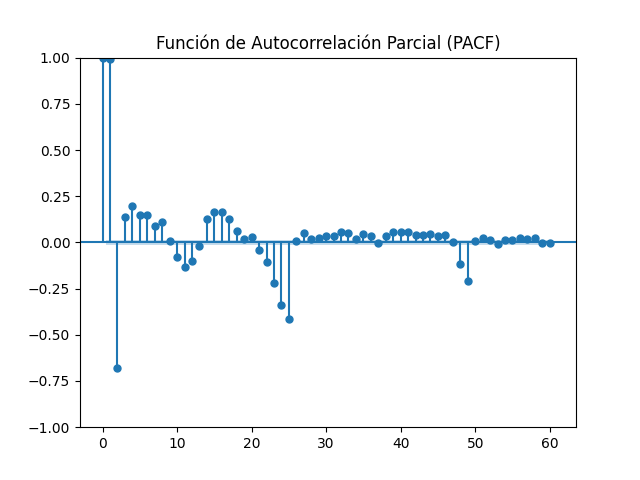
\includegraphics[width=0.5\textwidth]{images/arima_pacf_pres.png}
    \caption{Gráfico de PACF para la serie de presión atmosférica en La Laguna de Grafcan}
    \label{arima_pacf_pres}
\end{figure}


Analíticamente, se emplea el algoritmo descrito en \ref{pacf_ar_order}. Se determina $p$ = 4 para las series de temperatura del aire y humedad relativa, mientras 
que se obtiene $p$ = 8 en el caso de la presión atmosférica.

\begin{figure}[H]
    {\small
    \hrule \
    {\bf\small Pseudocódigo Selección de Orden AR vía PACF}
    \hrule
    \begin{center}
    \begin{tabbing}
    \ 1: {\bf Fun}\={\bf ción} seleccionar\_orden\_AR($serie$, $max\_lags$): \\
    \ 2: \> \# 1. Calcular la PACF hasta $max\_lags$ retardos \\
    \ 3: \> $pacf\_valores$ = PACF($serie$, $nlags$=$max\_lags$) \\
    \ 4: \> \# 2. Definir intervalo de confianza al 95\% \\
    \ 5: \> $intervalo\_confianza$ = 1.96 / raiz\_cuadrada(longitud($serie$)) \\
    \ 6: \> \# 3. Buscar el primer retardo no significativo \\
    \ 7: \> {\bf Para} \= $lag$ {\bf en} 1 \dots $max\_lags$: \\
    \ 8: \> \> {\bf Si} \= valor\_absoluto($pacf\_valores[lag]$) $<$ $intervalo\_confianza$: \\
    \ 9: \> \> \> imprimir("El mejor orden AR sugerido por la PACF es:", $lag-1$) \\
    \ 10: \> \> \> {\bf Retornar} $lag-1$ \\
    \ 11: \> \# 4. Si todos los retardos son significativos \\
    \ 12: \> imprimir("Todos los retardos hasta", $max\_lags$, "son significativos.) \\
    \ 13: \> {\bf Retornar} $max\_lags$ \\
    \end{tabbing}
    \end{center}
    \hrule
    }
    \caption{Pseudocódigo para Selección de Orden AR usando PACF}
    \label{pacf_ar_order}
\end{figure}

\subsection{Estudio de la estacionariedad}
Se emplea la prueba de Dickey-Fuller aumentada (ADF) para determinar la estacionariedad de las series temporales.
La prueba ADF es una prueba estadística que evalúa la presencia de una raíz unitaria en una serie temporal, lo que indica si la serie es estacionaria o no.
La hipótesis nula de la prueba ADF establece que la serie temporal tiene una raíz unitaria, lo que implica que no es estacionaria.
Si el valor p de la prueba es menor que un nivel de significancia predefinido (por ejemplo, 0.05), se rechaza la hipótesis nula y se concluye que la serie es estacionaria.

Empleamos como significancia un nivel de 0.05, y se observa que todas las series temporales son estacionarias, por lo que no es necesario aplicar diferencias, 
es decir, $d$ = 0.

\subsection{Determinación del orden de la media móvil}
Para calcular el número de términos de media móvil, se utiliza la función de Autocorrelación \texttt{ACF} de la librería \texttt{statsmodels}. Dicha función 
retorna los coeficientes de autocorrelación para diferentes retardos.

Analíticamente, se emplea el algoritmo descrito en \ref{acf_ma_order}, cuya idea principal consiste en comprobar para cada retardo si el 
coeficiente de autocorrelación es significativo, finalizando cuando se encuentra el primer retardo no significativo. 

Se calcula el intervalo de confianza como 1.96 por la raíz cuadrada de la longitud de la serie temporal, ya que la distribución de
la autocorrelación estimada en cualquier lag se aproxima a una distribución normal con media 0 y desviación estándar $\frac{1}{\sqrt{n}}$,
donde $n$ es el número de observaciones. De esta forma se obtiene un intervalo de confianza al 95\% para la autocorrelación. No obstante, se establece 
un límite inferior de 0.05 para evitar que el nivel de significancia sea demasiado bajo y se detecte el ruido como una señal significativa.
\begin{figure}[H]
    {\small
    \hrule \
    {\bf\small Pseudocódigo Selección de Orden MA vía ACF}
    \hrule
    \begin{center}
    \begin{tabbing}
    \ 1: {\bf Fun}\={\bf ción} seleccionar\_orden\_MA($serie$, $max\_lags$, $min\_confidence$): \\
    \ 2: \> \# 1. Calcular la ACF hasta $max\_lags$ retardos \\
    \ 3: \> $acf\_valores$ = ACF($serie$, $nlags$=$max\_lags$) \\
    \ 4: \> \# 2. Definir intervalo de confianza al 95\% \\
    \ 5: \> $intervalo\_confianza$ = max(1.96 / raiz\_cuadrada(longitud($serie$)), $min\_confidence$) \\
    \ 6: \> \# 3. Buscar el primer retardo no significativo \\
    \ 7: \> {\bf Para} \= $lag$ {\bf en} 1 \dots $max\_lags$: \\
    \ 8: \> \> {\bf Si} \= valor\_absoluto($acf\_valores[lag]$) $<$ $intervalo\_confianza$: \\
    \ 9: \> \> \> imprimir("El mejor orden MA sugerido por la ACF es:", $lag-1$)\\
    \ 10: \> \> {\bf Retornar} $lag-1$\\
    \ 11: \> {\bf Retornar} $max\_lags$\\
    \end{tabbing}
    \end{center}
    }
    \hrule
    \caption{Pseudocódigo para Selección de Orden MA usando ACF}
    \label{acf_ma_order}
\end{figure}

El algoritmo descrito retorna el máximo número de retardos para valores elevados de lags, por lo que se analiza el gráfico de la ACF y se observa que
no existe un punto de corte claro, sino que existe un descenso suave y progresivo para todas las variables \ref{acf_arima_temp} \ref{acf_arima_pres}. Por lo tanto, se fija $q$ = 0.

\begin{figure}[H]
    \centering
    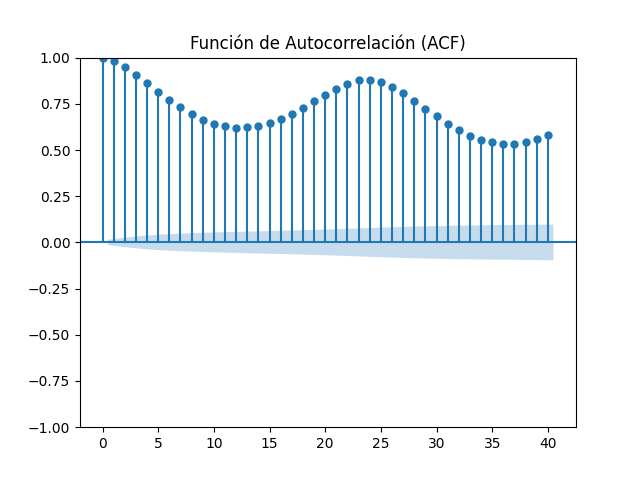
\includegraphics[width=0.5\textwidth]{images/arima_acf_temp.png}
    \caption{Gráfico de ACF para la serie de temperatura del aire en La Laguna de Grafcan}
    \label{acf_arima_temp}
\end{figure}

\begin{figure}[H]
    \centering
    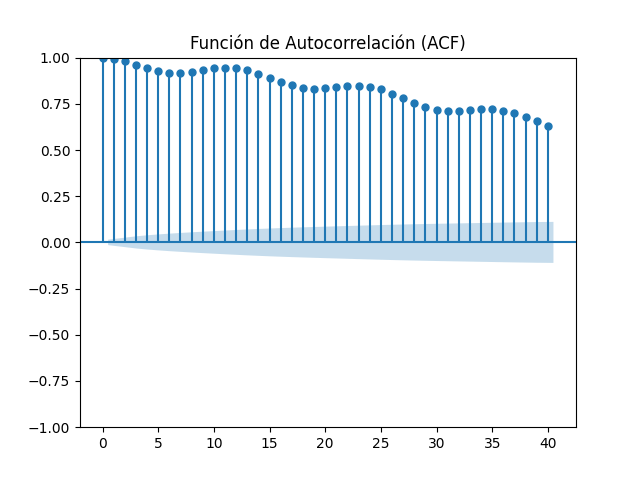
\includegraphics[width=0.5\textwidth]{images/arima_acf_pres.png}
    \caption{Gráfico de ACF para la serie de presión atmosférica en La Laguna de Grafcan}
    \label{acf_arima_pres}
\end{figure}

\subsection{Evaluación}
Para evaluar los modelos ARIMA empleamos la validación progresiva (walk-forward validation), que consiste en un bucle en el que se entrena al modelo, se realiza una predicción y se reentrena con los datos más recientes
antes de realizar la siguiente predicción. Este proceso se repite hasta que se alcanza el final del periodo de validación \ref{walk_forward_arima}. Emplearemos como métrica la raíz del error cuadrático medio (RMSE), 
que se calcula como la raíz cuadrada de la media de los errores al cuadrado entre las predicciones y los valores reales. Esta medición proporciona el error en la unidad de la variable.

\begin{figure}[H]
{\small
\hrule
{\bf\small Pseudocódigo Validación Walk-Forward con ARIMA}
\hrule
\begin{center}
\begin{tabbing}
\ 1: {\bf Fun}\={\bf ción} validacion\_walk\_forward($test$, $history$, $pasos\_prediccion$, $orden\_ARIMA$): \\
\ 2: \> $predicciones$ = lista\_vacía() \\
\ 3: \> $valores\_reales$ = lista\_vacía() \\
\ 4: \> {\bf Para} \= $t$ {\bf en} rango(0, longitud($test$) $-$ $pasos\_prediccion$ $+$ 1, $pasos\_prediccion$): \\
\ 5: \> \> $modelo$ = ARIMA($history$, orden=$orden\_ARIMA$) \\
\ 6: \> \> $ajuste$ = ajustar($modelo$) \\
\ 7: \> \> $pronostico$ = predecir($ajuste$, pasos=$pasos\_prediccion$) \\
\ 8: \> \> $predicciones$.añadir($pronostico$) \\
\ 9: \> \> $valores\_reales$.añadir($test[t : t+pasos]$) \\
\ 10: \> \> $history$.añadir($test[t : t+pasos]$) \\
\ 11: \> $rmse$ = raíz\_cuadrada(ECM($valores\_reales$, $predicciones$)) \\
\ 12: \> {\bf Retornar} $rmse$ \\
\end{tabbing}
\end{center}
}
\hrule
\caption{Pseudocódigo para validación walk-forward usando ARIMA}
\label{walk_forward_arima}
\end{figure}

Se toma como ejemplo la serie de temperatura del aire en Arona de Open-Meteo, con un horizonte de predicción de 3 horas. En la figura \ref{arima_residuals} se observan los residuos (diferencia entre valor real y predicción), mientras que en \ref{arima_residuals_density} se observa la estimación de la distribución de la densidad de los residuos.
Al estar centrada en 0 y tener una forma similar a la campana de Gauss, se puede concluir que el modelo ARIMA se ajusta bien a los datos. Finalmente, en la figura 
\ref{arima_results_graph} se muestra un ejemplo de los resultados obtenidos.

\begin{figure}
    \centering
    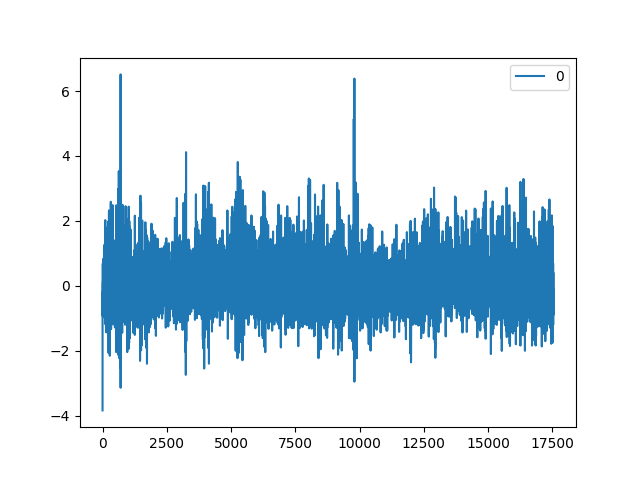
\includegraphics[width=0.7\textwidth]{images/arima_residuals.png}
    \caption{Residuos del modelo ARIMA para la serie de temperatura del aire en Arona de Open-Meteo}
    \label{arima_residuals}
\end{figure}

\begin{figure}
    \centering
    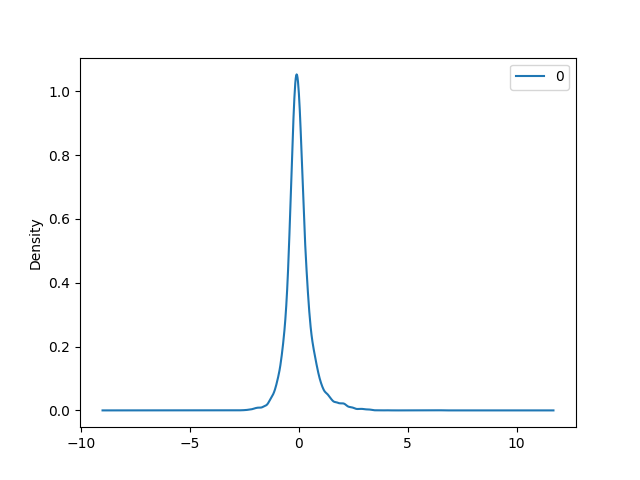
\includegraphics[width=0.7\textwidth]{images/arima_residuals_density.png}
    \caption{Distribución de los residuos del modelo ARIMA para la serie de temperatura del aire en Arona de Open-Meteo}
    \label{arima_residuals_density}
\end{figure}

\begin{figure}[H]
    \centering
    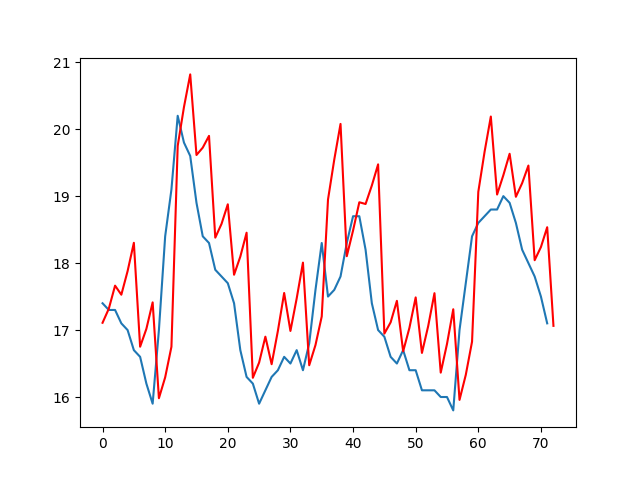
\includegraphics[width=0.7\textwidth]{images/arima_result.png}
    \caption{Resultados del modelo ARIMA para la serie de temperatura del aire en Arona de Open-Meteo}
    \label{arima_results_graph}
\end{figure}

\section{Modelos de aprendizaje profundo}
Existen diferentes frameworks para el desarrollo de modelos de aprendizaje profundo, destacando TensorFlow, PyTorch o JAX/Flax como los más extendidos.
Después de evaluar alternativas, se opta por TensorFlow debido a su amplia comunidad de usuarios y su extensa documentación, así como por su integración con Keras, 
una biblioteca de alto nivel que facilita la creación de modelos de aprendizaje profundo.

\subsection{Creación del dataset con TensorFlow}
Para crear el dataset, se emplea la función de TensorFlow \texttt{Dataset.from\_tensor\_slices()}, que permite crear un objeto Dataset 
a partir de tensores de entrada y salida. Dichos tensores son: la dupla (datos\_pasados, datos\_futuros) y el arreglo con los datos de validación.

Se crean dos datasets: uno para el entrenamiento y otro para la validación. Ambos se dividen en lotes (batches) de tamaño 64. Este número se elige tras realizar 
pruebas con diferentes tamaños de lotes en los distintos modelos, y se observa que, pese a ser un poco más inestable, ya que un número pequeño de muestras por lote
puede causar que el modelo cambie de forma exagerada en algún lote, con ese valor se consiguen los modelos con menor error. 

En el caso del conjunto de entrenamiento, tras crear los lotes se baraja, para evitar el sobreajuste y mejorar la generalización del modelo.

\subsection{Consideraciones generales}
Se emplea como métrica de pérdida el error mse de las ventanas de validación.

Además, para controlar el entrenamiento se emplean dos funciones de retorno (callbacks): 
\itemize{
\item \texttt{EarlyStopping}: detiene el entrenamiento si no se observa mejora en la métrica de validación durante un número determinado de épocas (patience). 
De esta forma se intenta evitar el sobreajuste. Además, se guarda el modelo con la mejor métrica de validación.
\item \texttt{ReduceLORonPlateau}: reduce la tasa de aprendizaje por un factor si no se observa mejora en la métrica de validación durante un número determinado de épocas (patience).
Se basa en la idea de que cuando el modelo no mejora, es posible que se encuentre cerca de un mínimo local y que una tasa de aprendizaje más baja pueda ayudar a acercarse más.
}

Para determinar estas variables, además de otros hiperparámetros como el ratio de aprendizaje, se hace uso de una herramienta de ajuste fino (fine-tuning). En particular, se emplea Keras Tuner, y el método de búsqueda
en rejilla (grid search), que consiste en definir un espacio de búsqueda para los hiperparámetros y evaluar todas las combinaciones posibles. Se realizan 5 ejecuciones por prueba y se 
emplea la media de los resultados.

\subsection{CNN}
Las redes convolucionales (CNN) son un tipo de red neuronal diseñadas originalmente para procesar datos con estructura de cuadrícula (como imágenes), pero también se pueden aplicar a series temporales (1D).
Su base es la convolución, una operación en la que uno o varios filtros (o núcleos) se deslizan sobre la entrada, calculando productos escalares para extraer características locales relevantes.
Cada filtro tiene un tamaño (kernel size) y avanza con un paso (stride) determinado; además, puede aplicarse padding (relleno) para controlar las dimensiones de la salida.
En una capa suelen existir múltiples filtros distintos, de manera que cada uno aprende a detectar un patrón diferente (por ejemplo, tendencias, picos o frecuencias concretas en series temporales).

Tras las capas convolucionales, es común intercalar capas de pooling (submuestreo), como max-pooling o average-pooling, para reducir dimensión, extraer características más robustas y controlar el sobreajuste.
Durante el entrenamiento de la red, los pesos de los filtros se ajustan para minimizar el error de predicción.

\subsection{LSTM}
Las redes LSTM (Long Short-Term Memory) son un tipo de red neuronal recurrente (RNN) que se utilizan para modelar secuencias temporales.
Las LSTM son capaces de aprender patrones a largo plazo en los datos, lo que las hace adecuadas para tareas de predicción de series temporales.
Se basan en la idea de utilizar celdas de memoria que pueden almacenar información durante períodos prolongados, lo que les permite recordar información relevante de entradas anteriores.
Cada unidad LSTM incluye una celda de memoria y tres puertas que regulan el flujo de información:
\itemize{
\item Puerta de entrada: decide qué información nueva se añade a la celda de memoria.
\item Puerta de olvido: determina qué información de la celda de memoria se olvida.
\item  Puerta de salida: controla qué información de la celda de memoria se envía como salida.
}

Son relevantes también las capas bidireccionales. Introducidas en 2005 por Graves y Schmidhuber \cite{graves_schmidhuber2005}, las LSTM bidireccionales permiten que la red procese la secuencia de 
entrada en ambas direcciones (hacia adelante y hacia atrás), lo que mejora la capacidad de capturar dependencias a largo plazo en los datos, ayudando, por ejemplo, a evitar
ambigüedades debido al mayor contexto.

\subsection{LSTM-CNN}
Los modelos híbridos LSTM-CNN combinan las ventajas de las redes LSTM y las redes convolucionales. Intercalan capas convolucionales y LSTM para capturar tanto patrones locales como dependencias a largo plazo en los datos de series temporales.
La arquitectura típica de un modelo LSTM-CNN incluye capas convolucionales iniciales para extraer características locales, seguidas de capas LSTM para capturar patrones temporales a largo plazo.

\section{Comparativa inicial}
Para establecer una referencia del rendimiento de los modelos neuronales, se compara un modelo LSTM con un modelo ARIMA, ambos con un horizonte de predicción de 3 horas.

Es difícil realizar una comparativa justa entre modelos ARIMA y de aprendizaje profundo, debido a que tienen naturalezas distintas.
Los ARIMA toman una serie temporal unidimensional para su entrenamiento, idealmente con un número elevado de observaciones (normalmente, más de 500),
 y generan una predicción de su continuación. Mientras que, con los modelos de aprendizaje profundo, buscamos crear un modelo capaz de predecir
una serie que no ha usado en su entrenamiento, a partir de una muestra pequeña, de menos de un día.  


Debido a estas limitaciones, los ARIMA se suelen evaluar sobre el periodo posterior al entrenamiento, lo que contrata con el enfoque de validación que habíamos implementado 
en los modelos neuronales, usando un muestreo aleatorio de las ventanas en todo el período contemplado.
Para comparar ambos modelos, se opta por emplear el mes de marzo de 2025, siendo ambos modelos entrenados con el intervalo de marzo de 2023 a febrero de 2025.  

En el caso de los modelos LSTM, se selecciona el mejor de 6 entrenamientos. 

Los resultados se muestran en la tabla \ref{comparativa_inicial}.

\begin{table}[ht]
\centering
\begin{tabular}{llrrrrrr}
\toprule
 &  & \multicolumn{2}{c}{Temperatura} & \multicolumn{2}{c}{Presión} & \multicolumn{2}{c}{Humedad} \\
\cmidrule(lr){3-4} \cmidrule(lr){5-6} \cmidrule(lr){7-8}
Ubicación & Fuente & ARIMA & LSTM & ARIMA & LSTM & ARIMA & LSTM \\
\midrule
\multirow{2}{*}{Arona}
  & Open-Meteo    & 1,088 & 0,630 & 0 & 0 & 0 & 0 \\
  & Grafcan & 1,263 & 0,697 & 0 & 0 & 0 & 0 \\
\addlinespace
\multirow{2}{*}{La Orotava}
  & Open-Meteo    & 0,917 & 0,496 & 0 & 0 & 0 & 0 \\
  & Grafcan & 1,344 & 0,832 & 0 & 0 & 0 & 0 \\
\addlinespace
\multirow{2}{*}{La Laguna 1}
  & Open-Meteo    & 0,806 & 0,385 & 0 & 0 & 0 & 0 \\
  & Grafcan & 0,902 & 0,699 & 0 & 0 & 0 & 0 \\
\addlinespace
\multirow{2}{*}{La Laguna 2}
  & Open-Meteo    & 1,157 & 0,497 & 0 & 0 & 0 & 0 \\
  & Grafcan & 1,049 & 0,621 & 0 & 0 & 0 & 0 \\
\addlinespace
\multirow{2}{*}{Santa Cruz}
  & Open-Meteo    & 0,806 & 0,404 & 0 & 0 & 0 & 0 \\
  & Grafcan & 1,335 & 0,832 & 0 & 0 & 0 & 0 \\
\addlinespace
\multirow{2}{*}{Garachico}
  & Open-Meteo    & 0,850 & 0,612 & 0 & 0 & 0 & 0 \\
  & Grafcan & 1,434 & 0,991 & 0 & 0 & 0 & 0 \\
\bottomrule
\end{tabular}
\caption{Comparativa inicial de modelos ARIMA y LSTM con predicciones de 3 horas} 
\label{comparativa_inicial}
\end{table}

TODO: Conclusiones.

A continuación, se comparan los modelos LSTM, CNN y el híbrido. En este caso, emplearemos el RMSE obtenido en la validación cruzada del entrenamiento.

\section{Estudios empíricos}
Se realizan diferentes experimentos sobre los modelos neuronales de cara a obtener el mejor rendimiento posible.

\subsection{Características de los modelos}
Se prueba el uso de diferentes elementos para evitar el sobreajuste y mejorar la generalización de los modelos, como las capas de abandono (dropout) y la normalización 
por lotes (batch normalization) o la normalización de capas (layer normalization). También se emplea el abandono recurrente, que consiste en aplicar el abandono a las conexiones recurrentes de la red LSTM, lo que ayuda a prevenir el sobreajuste al forzar a la red a aprender representaciones más robustas y generalizables.
Sin embargo, se observa que ninguna de estas técnicas mejora el rendimiento de los modelos, por lo que se opta por no incluirlas en las arquitecturas finales.

Por otra parte, también se evalúa el uso de conexiones residuales (residual connections) en las capas LSTM. Estas conexiones permiten que la salida de una capa no se sume a la
 entrada de otra capa no directamente adyacente (eg. dos capas por debajo), lo que ayuda a mitigar el problema de la desaparición del gradiente y facilita el entrenamiento de redes más profundas.
Se observa que su uso mejora ligeramente el rendimiento de los modelos, por lo que se opta por incluirlas en las arquitecturas finales.

Finalmente, se estudia el uso de capas de atención (attention layers) en los modelos LSTM. Introducidas por Bahdanau et al. \cite{bahdanau2014}, estas capas permiten que el modelo se enfoque en diferentes partes de la secuencia de entrada al hacer predicciones, lo que puede mejorar la capacidad del modelo para capturar patrones a largo plazo.
estas capas permiten que el modelo se enfoque en diferentes partes de la secuencia de entrada al hacer predicciones, lo que puede mejorar la capacidad del modelo para capturar patrones a largo plazo. Sin embargo, tras probar distintos tipos de atención en distintos puntos de la red, no se detecta mejora.

\subsection{Número de estaciones}
Se estudia el impacto del número de estaciones en la precisión de los modelos. Se entrena un modelo LSTM con diferente número de estaciones. Para evaluarlos, se mide el RMSE de validación de cada modelo.
Los resultados se muestran en la tabla \ref{estaciones_y_error}. Observamos que cuando se entrena utilizando 2 estaciones los resultados son peores que el promedio de ambas.
Esto puede explicarse porque cuando se entrenaba con una sola estación el modelo se especializaba en su comportamiento. Sin embargo, vemos que a medida que se añaden estaciones la 
diferencia entre los resultados del modelo entrenado con todas las estaciones y el promedio de cada estación se reduce, lo que refleja el aumento de la capacidad de generalización del modelo.

\begin{table}[h!]
\centering
\begin{tabular}{lcccc}
\toprule
\textbf{Ubicaciones} & \textbf{rmse} & \textbf{media} \\
\midrule
Arona                    & 0.6766677965 & \\
Orotava                  & 0.7597793601 & \\
La Laguna                & 0.5974298339 & \\
Punta Hidalgo            & 0.6190961388 & \\
Arona + Orotava          & 0.7563391658 & 0.7182235783 \\
Arona + Orotava + Laguna & 0.7068679189 & 0.6779589968 \\
TODOS                    & 0.6851888257 & 0.6632432823 \\
\bottomrule
\end{tabular}
\caption{Error de validación en función de las estaciones usadas}
\label{estaciones_y_error}
\end{table}

\subsection{Tamaño de la ventana}
Se estudia exhaustivamente el número de horas previas $P$ que contiene la ventana. Para ello, se construyen datasets desde $P$=6 hasta $P$=48 y se evalúan en los modelos 
desarrollados, eligiendo para cada valor de $P$ el mejor modelo de 5 entrenamientos. Se observan distintos valores óptimos de $P$ según las variables: $P$=17 para la temperatura del aire, $P$=24 para la humedad relativa y 
$P$=20 para la presión atmosférica. En la tabla \ref{window_size} se muestran los resultados obtenidos para el modelo LSTM y un horizonte de predicción de 3 horas,
en un gradiente en el que rojo indica el peor RMSE y verde el mejor.

\begin{figure}[H]
    \centering
    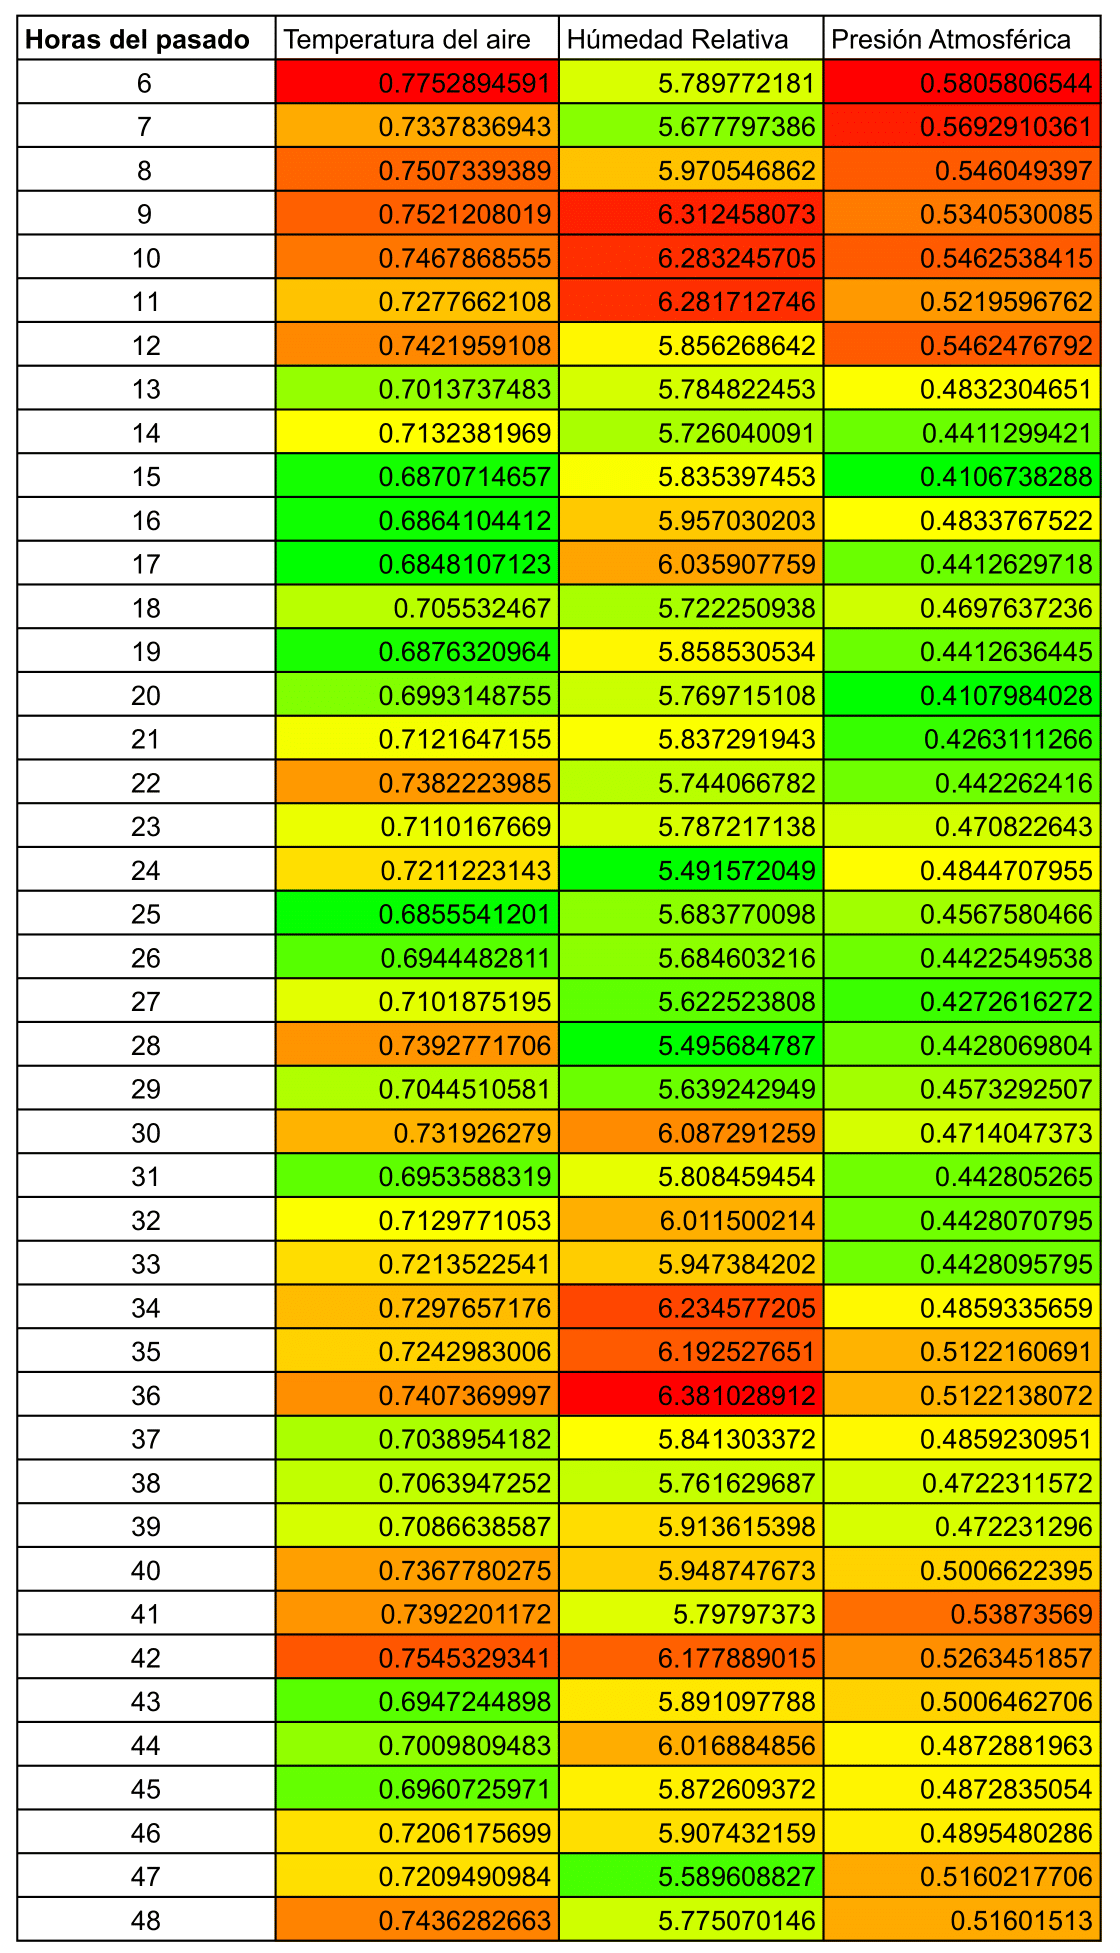
\includegraphics[width=0.7\textwidth]{images/past_window_size.png}
    \caption{Resultados del estudio del error RMSE del modelo LSTM en función del tamaño de la ventana }
    \label{window_size}
\end{figure}

Observando estos datos, se puede detectar un patrón en el que los modelos de 12 o menos horas dan peores resultados, 
mientras que el intervalo óptimo parece estar entre 15 y 26 horas, descendiendo los resultados a partir de las 30 horas.


\subsection{Uso de ruido}
Se plantea la hipótesis de que añadir un cierto ruido a los datos a medida que son consumidos en el entrenamiento puede favorecer la precisión del modelo al evitar el sobreajuste.
Esto es, se desea que el modelo en cada época no vea la misma muestra, sino que vea una versión ligeramente distinta. 

Para ello, se emplea el método .map del dataset de TensorFlow, que permite mapear otra función para su ejecución perezosa.
Se utiliza la función descrita en \ref{add_noise} sobre el conjunto de entrenamiento. En dicha función se aplica el ruido mediante una máscara
a los datos pasados de la variable y las covariables, sin alterar la codificación temporal. Además, se aplica ruido al valor objetivo $y$.

\begin{figure}[H]
{\small
\hrule
{\bf\small Pseudocódigo para agregar ruido}
\hrule
\begin{center}
\begin{tabbing}
\ 1: {\bf Función}\={\bf add\_noise}($x$, $y$, $covariates\_indexes$): \\
\ 2: \> Desempaquetar $x$ en \= $past,\, fut$ \\
\ 3: \> \# Generar ruido sobre las covariables \\
\ 4: \> $cov\_noise$ = noise\_distribution($past$, NOISE\_STD) \\
\ 5: \> \# Construir máscara de características afectadas \\
\ 6: \> $n\_features$ = shape($past$)[-1] \\
\ 7: \> $mask$ = ceros($(n\_features)$) \\
\ 8: \> $mask$[ $covariates\_indexes$ ] = 1 \\
10: \> $mask$ = reshape($mask$, $(1,1,n\_feat)$)  \# redimensión para aplicar al lote \\
11: \> \# Aplicar ruido sólo en características seleccionadas \\
12: \> $past\_noise$ = $cov\_noise \times mask$ \\
13: \> \# Generar ruido sobre la variable objetivo. \\
14: \> $target\_noise$ = noise\_distribution($y$, NOISE\_STD) \\
15: \> \# Retornar tupla con datos ruidosos y futuro sin modificar \\
16: \> {\bf Retornar}\ ( $(past + past\_noise),\, fut$ ),\ $y + target\_noise$ \\
\end{tabbing}
\end{center}
}
\hrule
\caption{Pseudocódigo de la función \texttt{add\_noise}}
\label{add_noise}
\end{figure}


Se prueban distintos valores de ruido y varias distribuciones: normal y una triangular, con menor desviación, construida mediante dos distribuciones uniformes.
Ejemplos de los datos con el ruido aplicado se pueden ver en las figuras \ref{noise1} y \ref{noise2}. También se experimenta aplicando coeficientes de ruido distintos a las covariables 
y a la variable objetivo. Se observa que un ruido menor al de las covariables en la variable objetivo mejora los resultados frente a usar el mismo valor.

\begin{figure}[H]
    \centering
    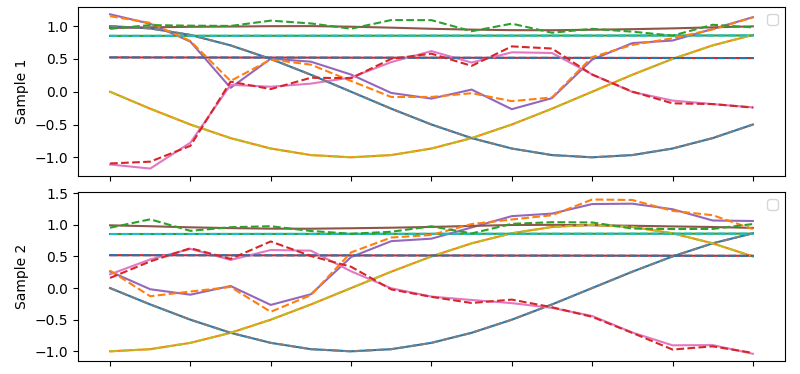
\includegraphics[width=0.7\textwidth]{images/noise_past_data.png}
    \caption{Datos pasados de 2 muestras. Datos originales en continua y con el ruido en discontinua.}
    \label{noise1}
\end{figure}

\begin{figure}[H]
    \centering
    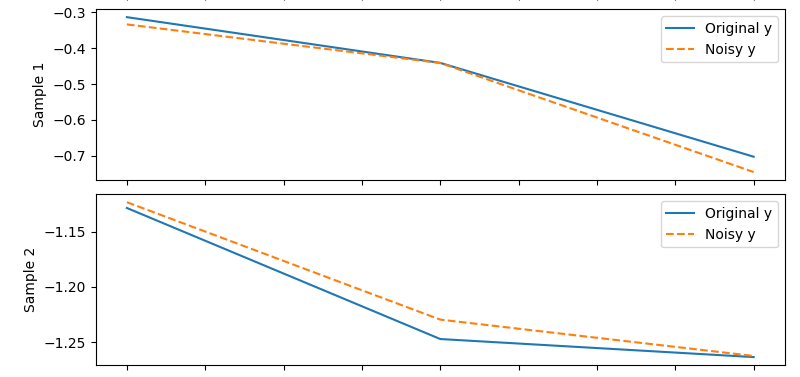
\includegraphics[width=0.7\textwidth]{images/noise_y.png}
    \caption{Valores objetivo de 2 muestras. Datos originales en continua y con el ruido en discontinua.}
    \label{noise2}
\end{figure}

Sin embargo, en la práctica se constata que el ruido no mejora los resultados de los modelos. Esto puede deberse a que las series exhiben una tendencia muy fuerte, 
que la inclusión del ruido no es capaz de modificar, puesto que sería necesario un ruido tan elevado que se perdería el valor de los datos.

\section{Modelos y Resultados}
\subsection{Temperatura del aire}
\subsection{Humedad relativa}
\subsection{Presión atmosférica}

